\chapter{Классификация известных методов восстановления изображений, искаженных дефокусировкой фотокамеры}

На рисунке 3.1 представлены критерии, согласно которым можно классифицировать существующие методы повышения качества изображений, искаженных дефокусировкой фотокамеры.~\cite{criteria}

\begin{figure}[!h]
	\center{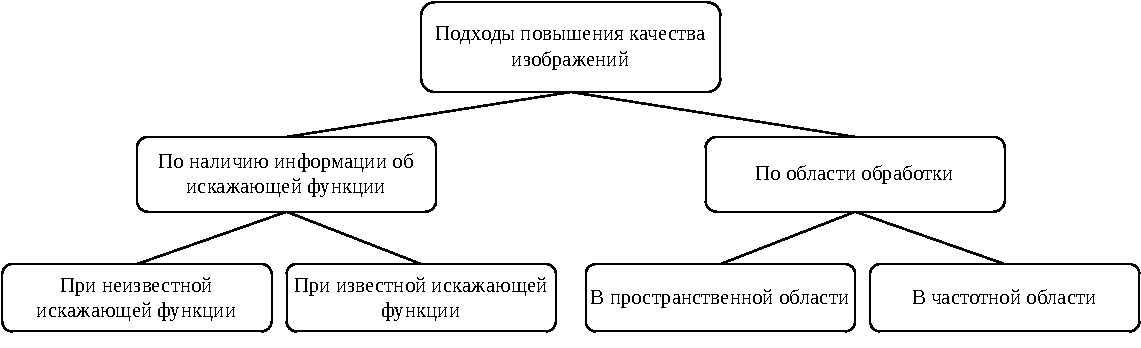
\includegraphics[scale=0.9]{assets/classification}}
	\caption{Классификация подходов повышения качества изображения}
\end{figure}

В таблице 3.1 представлен сравнительный анализ рассмотренных методов.

\renewcommand{\arraystretch}{2}
\begin{table}[h!]
	\begin{center}
	    \caption{Сравнительный анализ рассмотренных методов}
		""\newline
        \begin{adjustbox}{angle=0}
        \begin{tabular}{|c|c|c|}
        \hline
        \multirow{2}{*}{Метод} & \multicolumn{2}{c|}{Критерий} \\
        \cline{2-3}
        & \specialcell{Искажающая функция} & \specialcell{Область обработки} \\
        \cline{2-3}
        \hline
        \specialcell{Инверсная фильтрация} & Известна & Частотная\\
        \hline
        \specialcell{Фильтр Винера} & Известна & Частотная\\
        \hline
        \specialcell{Регуляризация Тихонова}  & Известна & Частотная\\
        \hline
        \specialcell{Метод Люси~--~Ричардсона} & Известна & Пространственная \\
        \hline
        \specialcell{<<Слепая>> деконволюция} & Неизвестна & Частотная\\
        \hline
        \end{tabular}
        \end{adjustbox}
\end{center}
\end{table}	

\clearpage

\section*{Вывод}

Таким образом, из рассмотренных методов только метод Люси~--~Ричардсона реализовывается в пространственной области, и только метод слепой деконволюции предполагает, что искажающая функция заранее неизвестна. 

Не существует универсального решения поставленной задачи. Алгоритм следует подбирать в зависимости от исходных данных и допущений, основываясь, например, на приведенной выше классификации. В практических задачах наиболее часто используется метод <<слепой>> деконволюции.



